\chapter{Realisieren}\label{ch:realisieren}
In diesem Kapitel wird die IPERKA-Phase Realisieren dokumentiert. Es werden die wichtigsten und entscheidendsten Punkte während der Implementierung festgehalten. 

\section{Backend erweitern}
In diesem Abschnitt wird die Implementierung des Backends dokumentiert. 
\subsection{Neuer REST-Endpunkt}
Als ersten Schritt wurde der neue REST-Endpunkt erstellt:
\begin{lstlisting}[language=Java]
	@JsonApiResource(attributes = Airlock2FAShortActivationCodeData.class)
@Path("activation-code-short")
public Response getShortActivationCode (@ExistingUser @PathParam("userId") @Parameter(schema = @Schema(type = "string")) UserParam userParam) {
	return ok(new Airlock2FAShortActivationCodeData(null)).build();
}
\end{lstlisting}
Der Endpunkt sieht aktuell so aus. Es sind noch keinerlei Funktionalitäten implementiert. Daher wird auch hardcoded null zurückgegeben. Airlock2FAShortActivationCodeData.java ist das DTO welches ein nullable Feld \flqq short\_activation\_code\frqq{} enthält. \\
\\
\textbf{Rolebased Access Control}\\
Damit der Zugriff auf den neuen Endpunkt nur dann funktioniert, wenn der Admin die nötigen Rollen dazu besitzt, musste eine neue RestAction definiert werden. Diese wird in der Klasse RestActionsDefinitions.java folgendermassen erstellt:
\begin{lstlisting}[language=Java]
	public static RestAction viewAirlock2FAActivationCode () {
	return RestAction
	.builder()
	.action(viewAirlock2FAActivationSecret)
	.rule(Rule.of(GET, "/users/[^/]+/tokens/airlock-2fa/activation-code-short"))
	.build();
}
\end{lstlisting}
Dies bewirkt nun, dass die Action \flqq viewAirlock2FASecrets\frqq{}, welche es schon gab, auf diesen Pfad matched. Das heisst bei jedem Call auf den neuen Endpunkt, wird zuerst validiert, ob der Nutzer die richtigen Rollen hat, welche für diese Action benötigt werden, ansonsten wird 403 zurückgegen.
Ein Problem hat sich nun hervorgehoben. Es gibt bereits folgendes Pattern:\\
 \flqq .rule(Rule.of(GET, "\verb*|text/users/[^/]+/tokens/airlock-2fa(/.*)?"))|\frqq{}
\\
Dieses Pattern matched auch auf den neuen Pfad. Da dieses Pattern in der allgemeine Action \flqq viewToken \frqq{} definiert wurde, könnte es nun zu Konflikten kommen. Deshalb wurde der neue Pfad in diesem Pattern mit Hilfe eines <<Negative Lookaheads>> ausgeklammert. Das neue Pattern für die viewToken Action sieht nun so aus:\\


\noindent \verb @/users/[^/]+/tokens/airlock-2fa(?!/activation-code-short(?:/|$))(/.*)?\$ @\\\\
So kann die viewAirlock2FAActivationSecrets Action unabhängig von der viewToken Action konfiguriert werden. Es entstehen dementsprechend keine Fehlkonfigurationen und Überschreibungen der Mappings.\\
\\
\textbf{REST-Dokumentation}\\
Eine Anforderung an neue REST-Endpunkte ist deren Dokumentation. Zum Zeitpunkt der Probe-IPA wird diese von Miredot via Javadoc generiert. Sprich Miredot erstellt eine REST-Dokumentation, basierend auf dem Javadoc. Für den neuen Endpunkt setzt sich diese Dokumentation wie folgt zusammen:
\begin{figure}[H]
	\begin{center}
		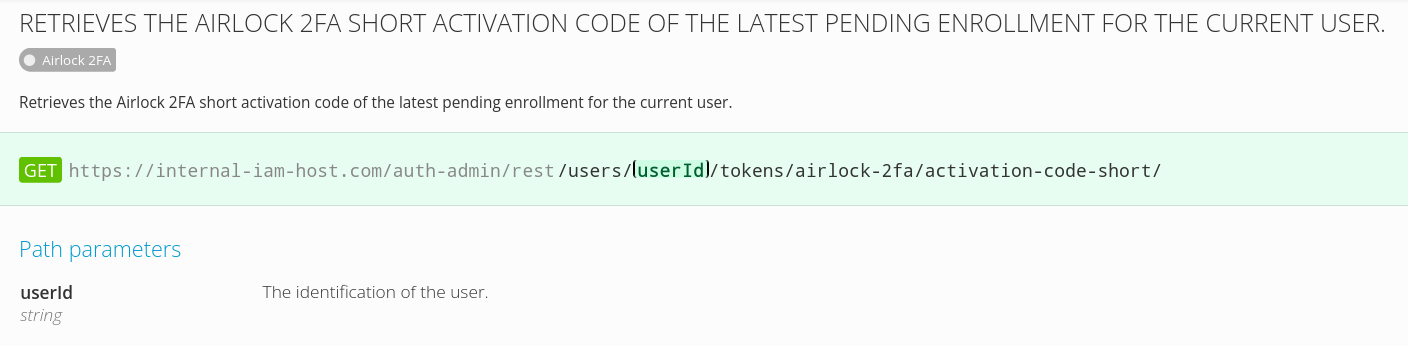
\includegraphics[width=1.0\textwidth]{ressourcen/requestdoc}
		\caption[REST-Dokumentation Request]{Miredot REST-Dokumentation Request}\label{fig:requestdoc}
	\end{center}
\end{figure}
\noindent Zu oberst ist immer der Titel des Requests. Darunter folgt eine Kurze Zusammenfassung. Danach ist der Pfad dargestellt mit der entsprechenden HTTP-Methode.
Zum Schluss folgen die Pfadparamter, was in diesem Fall die User ID ist.
Anschliessend folgt die Response:

\begin{figure}[H]
	\begin{center}
		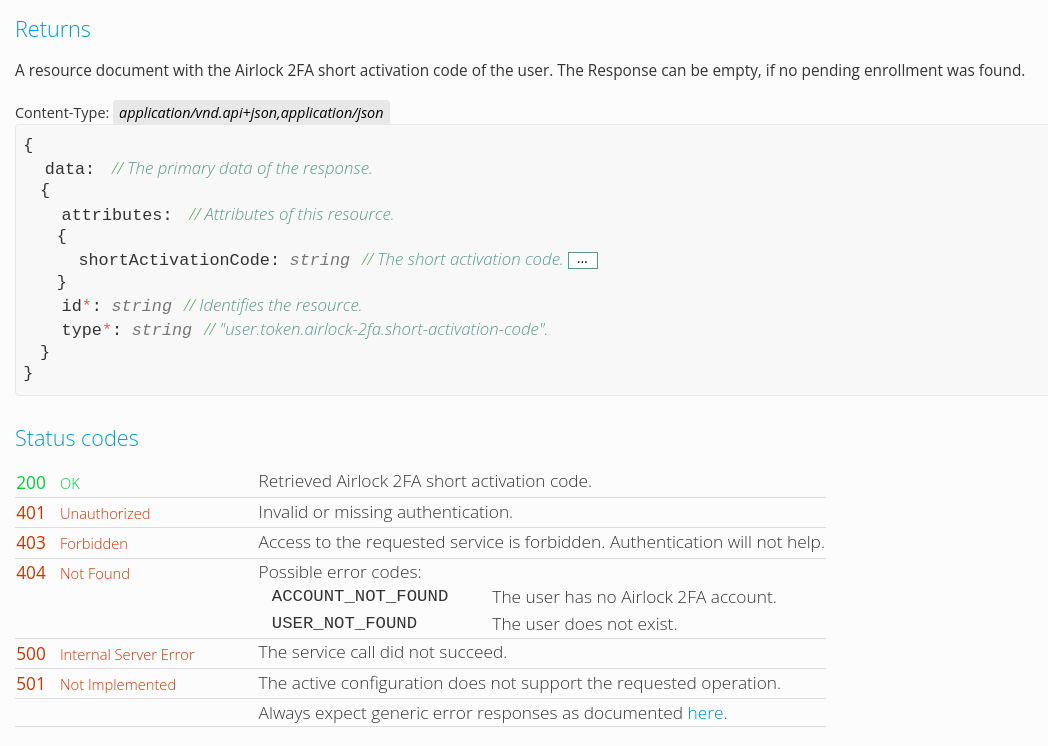
\includegraphics[width=1.0\textwidth]{ressourcen/responsedoc}
		\caption[REST-Dokumentation Response]{Miredot REST-Dokumentation Response}\label{fig:responsedoc}
	\end{center}
\end{figure}
\noindent Die Response der IAM-Endpunkte ist immer gleich aufgebaut. Sie verfügen über ein Data-Objekt, welches das Attributes-Objekt mit den jeweiligen geforderten Daten enthält. Nebst diesem Objekt hat es zwei weitere Felder, die Id, welche zur Identifizierung der Response gilt und zum anderen, der Type der Response. 
\subsection{Requests zu Futurae}\label{subsec:reqtofuturae}
Damit die SPA den 16-stelligen Aktivierungscode wie geplant angeboten bekommt, müssen in der Kommunikation zwischen IAM und Futurae einige Erweiterungen getroffen werden.\\
\\
\textbf{16-stelliger Aktivierungscode erzwingen}\\
Damit der 16-stellige Aktivierungscode bei dem Request, welcher das neuste offene Enrollment sucht, auch zurück kommt musste zuerst sichergestellt werden, dass bei dem Start-Enrollment-Request das Property \flqq shortcode\frqq{} auf true gesetzt wird. Dafür wurde auf dem Request Objekt ein weiteres Feld hinzugefügt.\\
Hier galt es zu beachten, dass jeweils 2 verschiedene Enrollment Requests gemacht werden:
\begin{itemize}
	\item Für einen neuen Nutzer, sprich ohne Account.
	\item Für einen Nutzer welcher schon einen Account besitzt. 
\end{itemize}
Dies musste sowohl für den Adminapp API Call zu Futurae als auch den Loginapp Call gemacht werden.
\\
\\
Nebst dem Request musste natürlich auch die Response geändert werden und um dieses Feld erweitert werden.
\\
Zum serialisieren und deserialisieren des Requests- / Response-Body wird Jackson verwendet. Dabei werden mit einfachen Annotationen die Java-Objekte auf die verlangten JSON-Felder gemapped oder umgekehrt:
\captionsetup[lstlisting]{labelformat=empty}
\begin{lstlisting}[language=Java, caption={Beispiel, wie Jackson auf dem Futurae Request zur Auth API (für die Self-Services) verwendet wird. (Enthält bereits das neue Feld \flqq short\_code\frqq{}).}]
@NoArgsConstructor
@Getter
@Setter
@JsonInclude(Include.NON_NULL)
public class FuturaeAuthApiEnrollmentRequest {
	
	@JsonProperty("user_id")
	private String userId;
	@JsonProperty("username")
	private String username;
	@JsonProperty("display_name")
	private String displayName;
	@JsonProperty("valid_secs")
	private Integer validSecs;
	
	@JsonProperty("short_code")
	private Boolean shortCode;
	
	@JsonProperty("success_callback_url")
	private String successCallbackUrl;
	@JsonProperty("phone_number")
	private String phoneNumber;
	@JsonProperty("enrollment_flow_binding_enabled")
	private Boolean enrollmentFlowBindingEnabled;
	@JsonProperty("account_recovery_flow_binding_enabled")
	private Boolean recoveryFlowBindingEnabled;
}
\end{lstlisting}
\newpage
\noindent\textbf{Erweitern der Requestfactory}\\
Als nächster Schritt wurde die FuturaeAdminApiEnrollmentRequestFactory.java um eine neue Methode erweitert:
\begin{lstlisting}[language=Java]
public RestRequest getLatestPendigEnrollment (String airlock2FAAccountId) {
	return futuraeRequestFactory.createGetRequest(ENROLLMENTS.usersPath(), getQueryParams(airlock2FAAccountId));
}

private static Map<String, Object> getQueryParams (String airlock2FAAccountId) {
	return Map.of("user_id", airlock2FAAccountId,
	"status", "pending",
	"sort_by", "created_at",
	"order", "desc",
	"limit", "1");
}
\end{lstlisting}
Diese Methode \flqq getLatestPendingEnrollment\frqq{} mit der statischen Hilfsmethode \flqq getQueryParams \frqq{} baut einen GET Request mit folgendem Pfad zusammen:\\\\
/srv/admin/v1/enrollments?user\_id={userid}
\newline\&status=pending 
\newline\&sort\_by=created\_at 
\newline\&order=desc
\newline\&limit=1\\\\
Dies ist der Request, welcher ausgeführt werden muss, um das neuste offene Enrollment zu bekommen.\\\\
\textbf{Erweitern des Enrollment Service}\\
Damit die Response von Futurae richtig geparst werden kann, musste zuerst ein äquivalentes Java Entity Objekt erstellt werden:
\begin{lstlisting}[language=Java]
@Data
@NoArgsConstructor
@AllArgsConstructor
@JsonIgnoreProperties(ignoreUnknown = true)
public class FuturaeAdminEnrollmentListResponse {
	
	@NotNull
	@JsonProperty("count")
	private Integer count;
	@NotNull
	@JsonProperty("enrollments")
	private List<FuturaeAdminEnrollmentResponse> enrollmentResponseList;
	@NotNull
	@JsonProperty("limit")
	private Integer limit;
	@NotNull
	@JsonProperty("offset")
	private Integer offset;
	@NotNull
	@JsonProperty("total")
	private Integer total;
}
\end{lstlisting}
Dieses Objekt bildet folgende JSON-Response, welche von Futurae so definiert wurde, in Java ab:
\begin{verbatim}
{
	"count": 0,
	"enrollments": [{FuturaeAdminEnrollmentResponse}],
	"limit": 0,
	"offset": 0,
	"total": 0
}
\end{verbatim}
Der FuturaeAdminApiEnrollmentServiceImpl.java ist die Schnittstelle zwischen IAM und Futurae, für alle Aktionen, welche das Enrollment betreffen. Für das wurde im seinem Interface die Methode \flqq getLatestPendingEnrollment\frqq{} definiert. Die Implementation sieht folgendermassen aus:
\begin{lstlisting}[language=Java]
@Override
public Optional<Airlock2FAEnrollment> getLatestPendingEnrollment (Airlock2FAAccountId accountId) {
	RestRequest request = 
	adminApiRequestFactory
	.getLatestPendigEnrollment(accountId.getId());
...
\end{lstlisting}
Zuerst wird der Request über die vorhin erstellte Methode zusammengestellt.
Danach wird er via den Restclient ausgeführt. Die Response wird anschliessend im folgenden Responsehandler behandelt:
\begin{lstlisting}[language=Java]
...
return restClient.read(request, response -> {
	if (response.getStatusInfo().equals(BAD_REQUEST)) {
		LOG.info("Invalid parameters for request to fecht latest pending enrollment for account with id: " + accountId.getId());
		return Optional.empty();
	}
	if (!response.getStatusInfo().equals(OK)) {
		LOG.info("Request to fetch the latest pending enrollment for account with id '" + accountId.getId() + "' failed with code: " + response.getStatusInfo());
		return Optional.empty();
	}
	FuturaeAdminEnrollmentListResponse result = readResponse(response, FuturaeAdminEnrollmentListResponse.class, request)
	.orElseThrow(Airlock2FAAdminApiException::new);
	if (result.getEnrollmentResponseList().isEmpty()) {
		LOG.info("Could not find a pending enrollment for account with id: " + accountId.getId());
		return Optional.empty();
	}
	LOG.info("Latest pending Enrollment fetched successfully for account with id: " + accountId.getId());
	return Optional.of(mapEnrollment(result
	.getEnrollmentResponseList().getFirst()));
});
\end{lstlisting}
Falls die Response einen 400 beinhaltet wird eine Info geloggt und Optional.empty zurück gegben. Dieser Fall sollte eigentlich nicht auftreten, es sei denn, das Futurae API ändert sich. Denn dieser Fehler kommt nur dann, wenn die Parameter falsch sind. Diese sind Hardcoded, können also nicht vom Nutzer beeinflusst werden. Um unerwartete Fehler zu vermeiden wird dieser Fall hier dennoch explizit abgefangen.\\
Da dies der einzige von Futurae definierte Error für diesen Request ist, werden die anderen mit dem darauf folgenden if-Statement abgefangen.\\
Danach wird in einem bereits bestehenden ResponseReader die Response in das Erwartete Objekt geparst. Ist das zurückkommende Result präsent, wird geprüft, ob es Einträge in der Enrollmentliste gibt. Falls ja wird ein Optional vom ersten Eintrag genommen. Dies geht, da man davon ausgehen kann, dass entweder genau 0 oder 1 Eintrag vorhanden ist. Dies weil im Request der <<limit>> -Parameter auf 1 gesetzt wurde.\\
\\
Dieses Optional wird dann über den Airlock2FAAdminService.java an die Resource überliefert, welche dann schlussendlich den 16-stelligen Aktivierungscode oder nichts, falls nichts vorhanden, als ResourceDocument zurückgibt.
\subsection{Logging}
Das Logging muss die Anforderung \flqq FA 3\frqq{} , definiert in Abschnitt \ref{subsec:anforderungenBackend}, erfüllen. Hierfür wurde im Airlock2FAAdminService.java folgende Methode imlementiert:
\begin{lstlisting}[language=Java]
	public Optional<String> findLatestPendingShortActivationCode (Airlock2FAUserAccount account) {
	return adminApiEnrollmentService
	.getLatestPendingEnrollment(account.getAccountId())
	.map(enrollment -> {
		signingLogger.log(format("Administrator '%s' accessed the Airlock 2FA short activation code of user '%s'.", administrator.getName(), account.getUserId()));
		helpdeskLogger.log(account.getUserId(), format("Administrator '%s' accessed the Airlock 2FA short activation code.", administrator.getName()));
		return enrollment.getActivationCodeShort();
	})
	.or(Optional::empty);
}
\end{lstlisting}
In dieser Methode wird aus dem erhaltenen Optional Enrollment der 16-stellige Aktivierungscode herausgefiltert und je nach Fall, ob präsent oder nicht, wird ein Optional String oder Empty zurückgegeben. Da dies der Service ist, welcher der Resource dient, in welcher der neue Endpunkt ist, wurde hier dann das Logging eingebaut. Das heisst diese Methode ist weniger allgemein, als jene im Enrollment-Service und es kann davon ausgegangen werden, dass sie nur für diesen Zweck verwendet wird. Der Signing Logger ist für das Audit Log, diese Message darf deshalb auch technisch sein und muss nicht für jeden verständlich sein.
Damit es auch im User Activities Logfile nachvollziehbar ist, welcher Admin wann auf einen Aktivierungscode zugegriffen hat, wurde der Helpdesklogger verwendet. In der Adminapp im Activities-Tab des aktuellen Nutzers, sieht dies nun wie folgt aus:
\begin{figure}[H]
	\begin{center}
		
\includegraphics[width=1.0\textwidth]{ressourcen/logpresent}
		\caption[Logeintrag bei vorhandenem Aktivierungscode]{Logeintrag bei vorhandenem Aktivierungscode}\label{fig:logpresent}
	\end{center}
\end{figure}
\noindent Im obigen Bild links, ist der Zeitpunkt, zudem der Admin auf den Code zugegriffen hat, zusehen. Auf der rechten Seite der Text, welcher im obigen Code im ersten Logstatement steht. 

\subsection{Resultat}
Die oben aufgezeigten Schritte führten schlussendlich zum gewollten Resultat. Der Endpunkt liefert nun den neusten, offenen Aktivierungscode, falls er vorhanden ist
\begin{verbatim}
{
	"meta": {
		"type": "jsonapi.metadata.document",
		"timestamp": "2024-11-14T13:12:29.093+01:00"
	},
	"data": {
		"type": "user.token.airlock-2fa.short-activation-code",
		"id": "2600345384",
		"attributes": {
			"shortActivationCode": "wdgj zjt4 m5h2 faxw"
		}
	}
}
\end{verbatim}
und sonst eine leere Response.
\begin{verbatim}
{
	"meta": {
		"type": "jsonapi.metadata.document",
		"timestamp": "2024-11-14T13:10:25.036+01:00"
	},
	"data": {
		"type": "user.token.airlock-2fa.short-activation-code",
		"id": "0",
		"attributes": {
			"shortActivationCode": ""
		}
	}
}
\end{verbatim}
Der Endpunkt ist durch den Role-Based Access Controller geschützt, sodass nur Admins mit den nötigen Rollen Zugriff haben. Alle anderen erhalten einen 403. Jeder erlaubte Zugriff wird nach den Anforderungen geloggt.
\subsection{Tests}\label{subsec:testbackend}
Die Unit-Tests so wie die Integration-Tests werden nach dem AAA(Arrange, Act, Assert)-Pattern gegliedert. Dies bedeutet, dass im ersten Abschnitt(Arrange) alles was für den Test gebraucht wird zusammengestellt wird. Im zweiten Abschnitt(Act) wird die zu testende Methode, resp. in den Integration-Tests der zu testende Endpunkt, aufgerufen. Und in einem dritten Abschnitt(Assert), wird das erwartete Resultat mit dem tatsächlichen Resultat verglichen. Dies dient der Übersicht und der Leserlichkeit des Tests. In einigen Fällen kann es sein, dass der erste Schritt weg fällt, da z.B nichts arranged werden muss, oder auf der Testklasse bereits arranged wurde. Nach jedem der Abschnitte kommt jeweils eine leere Zeile. \\
\\
\textbf{Ausbau Api Stubber}\label{head:stubber}\\
Wie in der Planung unter \ref{subsec:wiremock} bereits angesprochen, laufen die Tests nicht gegen das originale Futurae API, sondern gegen einen mit Wiremock simulierten Server.\\
Da der Endpunkt, der für den neuen Call zu Futurae (\ref{subsec:reqtofuturae}) angesprochen wird, auf dem Stubber noch nicht existiert, muss dieser zuerst erstellt werden. Dabei wird der Pfad definiert inkl. allen Queryparametern und der Response. Da als Response nicht immer das selbe erwartet wird, gibt es 2 verschiedene Methoden im Stubber:
\begin{lstlisting}[language=Java]
	public FuturaeAdminApiStubber withPendingEnrollmentList (String accountId, int limit) {
	wireMockClient.register(
	get(urlPathEqualTo(FUTURAE_ADMIN_ENROLLMENTS_PATH))
	.withQueryParams(getQueryParams(accountId, limit))
	.willReturn(aJsonResponse(
	defaultEnrollmentList(List.of(
	defaultEnrollment(DEFAULT_ACTIVATION_CODE)
	.activationCodeShort(DEFAULT_ACTIVATION_CODE_SHORT)
	.toJsonObject()), limit)
	.toJsonObject()))
	);
	return this;
}

public FuturaeAdminApiStubber withEmptyPendingEnrollmentList (String accountId) {
	wireMockClient.register(
	get(FUTURAE_ADMIN_ENROLLMENTS_PATH)
	.withQueryParams(getQueryParams(accountId, 1))
	.willReturn(aJsonResponse(emptyEnrollmentList()
	.toJsonObject()))
	);
	return this;
}

private static Map<String, StringValuePattern> getQueryParams (String airlock2FAAccountId, int limit) {
	return Map.of("user_id", equalTo(airlock2FAAccountId),
	"status", equalTo("pending"),
	"sort_by", equalTo("created_at"),
	"order", equalTo("desc"),
	"limit", equalTo(valueOf(limit)));
}
\end{lstlisting}
Die erste gibt eine Response, welche erfolgreich ist zurück. Die zweite eine Response in der die Enrollment Liste leer ist, heisst es wird simuliert, dass kein offenes Enrollment existiert. Diese 2 Fälle reichen aus, um das neue Feature zu testen.
Dieser Stubber wird für alle REST-Integration-Tests verwendet. Für die Unit-Tests wird direkt im Test gestubbed. Das Prinzip ist aber das gleiche.\\\\
\textbf{Integration-Tests}\label{header:inttest}\\
Für die Integration-Tests ist wichtig, dass eine IAM-Instanz läuft. In jedem Test wird eine IAM-Konfiguration zusammengestellt, welche die für die Tests notwendigen Plugins einkonfiguriert hat:
\begin{lstlisting}[language=Java]
private IamConfig adminApp (String allowedToViewAirlock2FAActivationSecrets) {
	return iamConfig()
		.newAdminapp()
		.addRoleBasedAccessControl(roleBasedAccessControl()
			.viewAirlock2FAActivationSecret(
			allowedToViewAirlock2FAActivationSecrets))
		.withStartPages(MANAGE_USER)
		.addTokenController(
			airlock2FATokenController(futuraeApiUrl)
			.build())
		.build();
}
\end{lstlisting}
In diesem Fall sieht es so aus.  Diese Methode hat einen Parameter um die Role Based Access Control je nach Testcase zu beeinflussen.
Vor jedem Test wird nun diese Config geladen und Aktiviert, es sei denn, es werden Custom Configs verwendent. Dieser Fall ist in Kaptitel \ref{subsec:testacc} beschrieben.\\
Hier ist ein Beispiel wie die zuvor erstellten Stubbermethoden in einem Test genutzt werden können:
\begin{lstlisting}[language=Java]
@Test
void shouldGetAirlock2FAShortActivationCode (FuturaeAdminApiStubber stubber) {
	addAirlock2FAAccount(DEFAULT_USERNAME);
	stubber.withPendingEnrollmentList(defaultAccount().userId().toString(), 1);
	
	JsonApiResourceResponse<Airlock2FAShortActivationCodeAttributes> response = getAirlock2FAShortActivationCode(DEFAULT_USERNAME);
	
	assertThat(response)
	.satisfies(r -> {
		assertThat(r.getData().getAttributes()).isNotNull();
		String actualCode = r.getData().getAttributes().getShortActivationCode();
		assertThat(actualCode).isNotNull();
		assertThat(actualCode)
		.isEqualTo(DEFAULT_ACTIVATION_CODE_SHORT);
	})
	.hasStatus(OK);
}
\end{lstlisting}
Zuerst wird ein neuer Airlock2FA Account hinzugefügt. Danach kommt die neue Stubbermethode zum Einsatz. Sie registriert auf dem Server den in der Methode definierten Endpunkt. Der Test macht danach den Call auf den neuen Endpunkt im IAM. Dieser löst dann den Request zum Mock-Server aus, welcher die definierte Response liefert. Am Schluss wird die Response, des IAM-Endpunktes, verifiziert. So kann sichergestellt werden, ob der neue Endpunkt wie erwartet funktioniert.\\
\\
\textbf{Unit-Tests}\\
Für den Unit-Test des FuturaeAdminApiEnrollmentServiceImpl.java musste der Futurae Server auch gemockt werden. Denn, die Aktionen dieses Services sind von den Antworten des Futurae Servers abhängig.
\begin{lstlisting}[language=Java]
@Test
void getLatestPendingEnrollmentShouldBeEmtpy () {
	withEnrollmentListResponse(EXISTING_FUTURAE_USER_ID.getId(),
	aJsonResponse()
	.withBody(emptyEnrollmentList()));
	
	Optional<Airlock2FAEnrollment> enrollmentOptional = adminApiEnrollmentService()
	.getLatestPendingEnrollment(EXISTING_FUTURAE_USER_ID);
	
	assertThat(enrollmentOptional).isEmpty();
	
}
\end{lstlisting}
Das obige Beispiel zeigt einen Unit-Test welcher sicherstellt, dass falls von Futurae eine Response ohne Enrollments zurück kommt, die Response der neuen Methode wie erwartet Optional Empty zurück gibt.\\
Für die Unit-Tests des Airlock2FAAdminService.java konnte schon der\\
Airlock2FAAdminApiEnrollmentService.java gemockt werden, das heisst hier war Wiremock nicht mehr nötig. Nebst dem richtigen Resultat wurde in diesen Tests, auch das Logging getestet. Mit der Hilfe von Mockito.verify konnte einfach verifiziert werden, ob die Logger die erwarteten Statements geloggt haben:
\begin{lstlisting}[language=Java]
verify(signingLogger).log("Administrator 'admin' accessed the Airlock 2FA short activation code of user 'user'.");
verify(helpdeskLogger).log(account.getUserId(), "Administrator 'admin' accessed the Airlock 2FA short activation code.");
\end{lstlisting}
\subsection{Testen der Access Control}\label{subsec:testacc}
Um mit automatisierten Tests sicherzustellen, dass nur berechtigte Admins Zugriff auf den 16-stelligen Aktivierungscode haben, musste zuerst die Konfiguration im REST-Integration-Test angepasst werden. Hierfür wurde zuerst im <<AdminappConfigBuilder.java>> eine neue Methode hinzugefügt, damit man die Role Based Access Controller Config dynamisch setzen kann. Danach musste diese im Test konfiguriert werden. Da es je nach Test eine andere Konfiguration der berechtigten Rollen braucht, musste dies dynamisch mit Parameter und Custom Configs gelöst werden. Das bedeutet, die Default-Config hat den Wert \flqq superadmin\frqq{}. Dies erlaubt dem Default-User den Zugriff auf die Airlock2FA Activation Secrets. Um zu testen, ob ein Admin ohne die Erforderliche Rolle auch wirklich kein Zugriff hat, kann man nun in diesem Test die Konfiguration bearbeiten und manuel aktivieren:
\begin{lstlisting}[language=Java]
@Test
@CustomConfig
void shouldGet403IfAccessNotAllowed () {
	adminApp("helpdesk").activate();
	addAirlock2FAAccount(DEFAULT_USERNAME);
	
	var response = getAirlock2FAShortActivationCode(DEFAULT_USERNAME);
	
	assertThat(response).hasStatus(FORBIDDEN);
}
\end{lstlisting}
Damit der Rest der Konfiguration gleich bleibt, wurde nur der Inhalt des Rollenfelds, für die Action \flqq viewAirlock2FAActivationCode\frqq{} als Parameter definiert. Hier wird jetzt die Default-Config überschrieben und der Inhalt auf <<helpdesk>> gesetzt. Da der Adminnutzer in diesem Test nur die Rolle superadmin hat, wird der Status FORBIDDEN erwartet.
\section{SPA erweitern}
Im folgenden Abschnitt wird beschrieben wie die Adminseite in der SPA erweitert wurde.

\subsection{Request zur IAM API}
Zuerst wurde ein neues Model erstellt, welches auf die JSON-Response gemapped werden kann:
\begin{lstlisting}[language=TypeScript]
export class Airlock2FAShortActivationCode {
	activationCodeShort: string;
}
\end{lstlisting}
Im Rahmen der Probe-VA ist dies ein Objekt mit einem string-Property, welches den 16-stelligen Aktivierungscode abbildet. \\
Danach wurden die Funktionalitäten eingebaut, um den neuen Endpunkt aus der SPA anzusteuern. Dazu wurde der \flqq airlock-2fa.service.ts\frqq{} um folgende 2 Methoden erweitert:
\begin{itemize}
	\item getLatestPendingActivationCode: Diese Methode führt den Request, mit Hilfe des Http Client aus dem Angular <<common>> Package, aus. 
	\item toAirlock2FAShortActivationCode: Dies ist die Mapper-Methode, welche die JsonApiResponse ausliest und in ein neues Objekt, des zuerst erstellten Model's, parsed. 
\end{itemize}
Dieses Objekt wird schlussendlich von der ersten Methode \flqq getLatestPendingActivationCode\frqq{} zurückgegeben.

\subsection{Darstellung im UI}
Damit der 16-stellige Aktivierungscode wie erwartet im Popup angezeigt wird, musste die bestehende <<airlock-2fa>>-Komponente im HTML für die Struktur und im Typescript für die Logik, erweitert werden.
\\
\\
\textbf{airlock-2fa.component.html}
\\
Zuerst wurde das HTML erweitert. Es wurde der neue Button hinzugefügt, welcher das Popup triggert:
\begin{lstlisting}
<iam-button
	*ngIf="isCodePresent"
	[id]="viewShortActivationCodeButtonId"
	[hideOnAccessDenied]="true"
	[text]="'Activation code'"
	[right]="true"
	[outsideOfCard]="true"
	(buttonClick)="viewActivationCode()">
</iam-button>
\end{lstlisting}
Ohne Implementation des Typescript's funktioniert dieser Button natürlich noch nicht.\\
\\
\textbf{airlock-2fa.component.ts}
\\
Im Typescript wurde die ganze Logik des Buttons implementiert. Sprich, wann darf er angezeigt werden und was passiert, wenn man in anklickt. \\
Damit sichergestellt wird, dass der Button nur angezeigt wird, wenn der Admin auch die erforderlichen Rollen hat, gibt es auf der <<iam-button>> Komponente ein Feld, namens \flqq hideOnAccessDenied\frqq{}. Wird dieses Feld auf true gesetzt, wird der Button nur angezeigt, wenn, die in Airlock2FATokenPermissions.java definierte Action, für diesen Button von dem Access Controller für diesen Admin erlaubt wird:
\begin{lstlisting}[language=Java]
private void addActivationCodePermissions (PagePermissionsBuilder page) {
	page.permission("viewShortActivationCode", accessController
	.isActionAllowed(viewAirlock2FAActivationSecret));
}
\end{lstlisting}
Dieses Mapping funktioniert über die Button-ID. Sprich der Key der Permisson muss den selben Stringwert haben, wie die ID des Buttons. Doch wie in der Anforderung \flqq FA 8\frqq{} in Kapitel\ref{subsec:anforderungenSPA} beschrieben, sollte der Button auch nur angzeigt werden, falls auch ein offener Aktivierungscode existiert. Für das wird in der ngOnInit-Methode, falls der Admin die nötigen Rollen hat, der Request ausgeführt, und falls die Response nicht leer ist, das boolean-Flag \flqq isCodePresent auf true gesetzt. Um den Request auszuführen wird die zuvor im Service erstellte Methode aufgerufen. Der 16-stellige Aktivierungscode wird bewusst nicht im ngOnInit lokal in die Komponente gespeichert, da es sein kann, dass er plötzlich nicht mehr offen ist, oder nicht mehr der neuste ist. Der Aktivierungscode wird deshalb immer neu angefragt wenn der Button geklickt wird. Mit anderen Worten, im ngOnInit wird nur validiert, ob der Button angezeigt werden darf oder nicht. Wird der Button geklickt, führt er folgene Methode aus:
\begin{lstlisting}[language=TypeScript]
viewActivationCode () {
	this.findPendingActivationCode().subscribe(
	res => {
			this.pageDialog.show({
				showCancel: false,
				okText: 'Close',
				title: '16-digit activation code',
				text: this.isCodePresent ?
					this.languageService
					.translate('Activation code:')
					+ ' '
					+ res.activationCodeShort :
					'Code is not pending anymore.'
			});
		}
	);
}
\end{lstlisting}
Diese führt zuerst wieder den Request aus. Sobald eine Antwort zurück kommt, wird der Dialog angezeigt. Das Aussehen und Verhalten des Dialog's kann ein Stück weit über die PageDialogSettings, welche der show-Methode übergeben werden, beeinflusst werden. So sorgt bspw. <<showCancel: false>> dafür, dass nur der Ok Button angezeigt wird, welcher bei einem Klick, das Popup schliesst. Die PageDialog Komponente existierte bereits. Jedoch hatte sie gerade bei diesem Feld noch einen Bug, welcher noch nicht entdeckt wurde, da dieses Feld noch nirgends, versucht worden ist zu überschreiben. Das Problem war folgendes:\\
Die Booleans wurden in der <<show>>-Methode bisher wie folgt versucht zu überschreiben:
\begin{lstlisting}[language=TypeScript]
this.showCancel = settings.showCancel || true;
\end{lstlisting}
Dies hat zwar für alle Stringvalues gut funkioniert, denn bei einem String kann so direkt geprüft werden, ob er undefined, empty oder null ist. Falls ja, wird der Defaultwert verwendet.
Bei einem Boolean funktioniert das nicht, da dieser false als einen gültigen Wert hat. Sprich setzt man showCancel beim Aufruf auf false, wird hier automatisch true verwendet. Dies weil das erste Statement false ist und der Operator || auf falsy-Werte prüft, welches unteranderem auch der Wert false ist. Die Lösung für dieses Problem war, dass man den Boolean mit dem Nullish Coalescing Operator <<??>> explizit nur auf null und undefined prüft, und nicht auf andere falsy Werte, wie false:
\begin{lstlisting}[language=TypeScript]
this.showCancel = settings.showCancel ?? true;
\end{lstlisting}
Also falls dieses Flag nicht von aussen gesetzt wird, dann ist es undefined, und wird auf den Standartwert true gesetzt. Ansonsten, falls es von aussen gesetzt wird, wird dieser Wert verwendet.
\\
Der Inhalt des Dialogs, wird über das erforderliche Feld \flqq text\frqq{} gesetzt. Hier wird dann die Antwort aus dem Request, sprich der 16-stellige Aktivierungscode, eingefüllt und somit im Popup angezeigt.
\begin{lstlisting}[language=TypeScript]
text: 'Activation code:'
		+ ' '
		+ res.activationCodeShort

\end{lstlisting}
Falls nun der Button geklickt wird, der Aktivierungscode aber im Hintergrund bereits nicht mehr offen ist, wird dies in Form von einem Page-Alert gelöst:
\begin{lstlisting}[language=TypeScript]
this.pageAlertService.error('The activation is not pending anymore.').display();
\end{lstlisting}
Dieser Alert sieht im UI dann so aus:
\begin{figure}[H]
	\begin{center}
		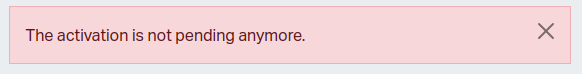
\includegraphics[width=1.0\textwidth]{ressourcen/pagealert}
		\caption[Page Alert]{Page Alert, falls der Aktivierungscode bereits nicht mehr offen ist.}\label{fig:pagealert}
	\end{center}
\end{figure}

\subsection{i18n Translation Keys}
Da die Admin-App die 3 Sprachen, Deutsch, Englisch und Französisch unterstützt, können die Texte nicht, so wie sie aktuell sind, <<hardcoded>> gesetzt werden. Alle Texte, also Titel, Popuptext oder der Text im Button, müssen über Translation Keys verfügen. Für jede Sprache gibt es ein JSON-File, welches zu diesen Keys jeweils den richtig übersetzten Wert hat. Mithilfe des Language Service, können diese dann auf die gewünschte Sprache eingefügt werden. Das Json für die deutsche Sprache sieht so aus:
\begin{verbatim}
{
...
"user": {
		...
		"airlock-2fa"{
			...
			"activation": {
				"view-activation-code": {
					"button": "Aktivierungs-Code anzeigen",
					"popup": {
						"close": "Schliessen",
						"title": "16-stelliger Aktivierungs-Code",
						"text": {
							"code": "Aktivierungs-Code:",
							"not-pending": "Die Aktivierung ist nicht mehr offen."
						}
					}
				}
			}
		}
	}
}
	

\end{verbatim}
Dies ist die Struktur für die folgenden Keys:
\begin{itemize}
	\item user.airlock-2fa.activation.view-activation-code.button
	\item user.airlock-2fa.activation.view-activation-code.popup.close
	\item user.airlock-2fa.activation.view-activation-code.popup.title
	\item user.airlock-2fa.activation.view-activation-code.popup.text.code
	\item user.airlock-2fa.activation.view-activation-code.popup.text.not-pending
\end{itemize}
Am Beispiel des Popup Textes sieht man, wie diese verwendet werden:
\begin{itemize}
	\item Ohne Keys:
	\begin{lstlisting}[language=TypeScript]
	text:'Activation code:'
		+ ' '
		+ res.activationCodeShort
		
	\end{lstlisting}
	\item Mit Keys:
	\begin{lstlisting}[language=TypeScript]
   	this.languageService
        .translate('user.airlock-2fa.activation
        	.view-activation-code.popup.text.code')
	+ ' '
	+ res.activationCodeShort
	\end{lstlisting}	
\end{itemize}
Im tatsächlichen UI sieht das ganze mit den Keys schlussendlich so aus:
\begin{figure}[H]
	\begin{center}
		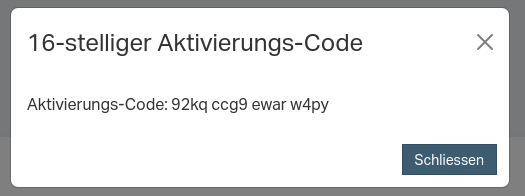
\includegraphics[width=1.0\textwidth]{ressourcen/popup-de}
		\caption[Popup deutsch]{Popup deutsch}\label{fig:popup-de}
	\end{center}
\end{figure}
\begin{figure}[H]
	\begin{center}
		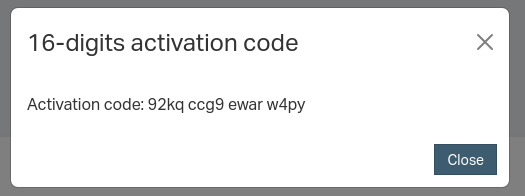
\includegraphics[width=1.0\textwidth]{ressourcen/popup-en}
			\caption[Popup englisch]{Popup englisch}\label{fig:popup-en}
	\end{center}
\end{figure}	
\begin{figure}[H]
	\begin{center}
		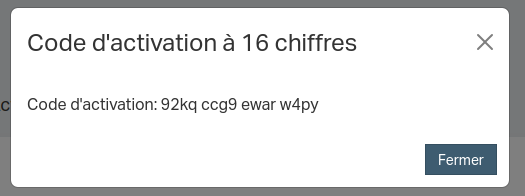
\includegraphics[width=1.0\textwidth]{ressourcen/popup-fr}
		\caption[Popup französisch]{Popup französisch}\label{fig:popup-fr}
	\end{center}
\end{figure}
\noindent Wie man sieht, wird der Text im Popup nun immer auf die aktive Sprache der SPA übersetzt.
\subsection{UI Integration-Tests}
Die UI Integration-Tests werden im IAM mit der Hilfe von Selenium durchgeführt. Durch dies wird das komplette Feature von der SPA bis zum Backend / der DB (Futurae (Wiremock)-Server) und wieder zurück getestet. \\
Wie bei den REST-Integration-Tests braucht es auch bei den UI-Integration-Tests für jeden Tests eine Config und einen Default User. In diesem Fall sind diese dieselben wie in Kapitel \ref{header:inttest} beschrieben.
\newpage
\noindent \textbf{Java Component erweitern}\\
Damit die Testklasse frei von Seleniumlogik bleibt, werden die einzelnen SPA-Seiten in separaten Klassen abgebildet. Diese Klassen beinhalten die notwendigen Methoden mit den passenden Selektoren, um auf der Seite zu navigieren und die Seite zu asserten. Diese Methoden werden dann von den Testklassen aufgerufen. Für das neue Popup wurde, eine neue Dialog Component erstellt. Sie besitzt folgende Methoden:
\begin{itemize}
	\item assertNoCancelButton()
	\item assertCloseButton()
	\item assertShortActivationCode(String shortActivationCode)
	\item clickCloseButton()
\end{itemize}
Mit Hilfe dieser Methoden konnte das ganze Popup getestet werden. Das Prinzip der Methoden ist immer das selbe. Sie selektieren ein HTML-Element mit einem Selektor erbend vom Typ \flqq By\frqq{}. Auf dem selektierten Element wird dann die gewünschte Aktion durchgeführt. Bspw: assertShortActivationCode(String shortActivationCode):
\begin{lstlisting}[language=Java]
public Airlock2FAShortActivationCodeDialogComponent assertShortActivationCode (String shortActivationCode) {
	assertTagWithIdContains("pageDialog", translate("user.airlock-2fa.activation
	.view-activation-code.popup.text.code") 
	+ " " 
	+ shortActivationCode);
	return this;
}
\end{lstlisting}
Hier wird der HTML-Tag mit der ID \flqq pageDialog\frqq{} selektiert. Dies entspricht dem Popup-Element. Danach wird verglichen, ob der Wert welcher im JSON-Key steht, plus der erwartete Aktivierungscode, auch wirklich im Popup enthalten sind. Schlussendlich wird die aktuelle Component wieder zurück gegeben, um weitere Aktionen darauf zu tätigen.
\\
Nebst dieser neuen Dialog Component, muss die UserDetailsAirlock2FATabComponent.java auch noch um 3 Methoden erweitert werden, da der Button um das Popup zu öffnen auf dieser Component ist:
\begin{itemize}
	\item assertViewShortActivationCodeButtonPresent()
	\item clickViewActivationButton()
	\item reload()
\end{itemize}
\textbf{Refactoring API Stubber}\\
Im Rahmen der Selenium Tests wurden die Methoden im API-Stubber, welche im Abschnitt \ref{head:stubber} erstellt wurden, umgebaut. Den für die UI-Integration-Tests muss es möglich sein, für einen einzelnen Test, sprich den selben Stubber, den gleichen Endpunkt auf verschiedene Arten zu simulieren. Deshalb wurde auf der Stubber Klasse ein neues Feld \flqq private Optional<MappingBuilder> pendingEnrollmentList; \frqq{} hinzugefügt. Dieses Feld enthält immer die aktuelle Version des Endpunktes. Danach wurde eine neue Methode hinzugefügt: 
\begin{lstlisting}[language=Java]
private void withPendingEnrollmentList (MappingBuilder newEnrollmentListMapping) {
	if (pendingEnrollmentList.isPresent()) {
		wireMockClient
		.removeStubMapping(pendingEnrollmentList.get());
	}
	pendingEnrollmentList = Optional.of(newEnrollmentListMapping);
	wireMockClient.register(newEnrollmentListMapping);
}
\end{lstlisting}
Diese Methode wird nun von den beiden bisherigen Methoden aufgerufen, jedoch mit anderen Endpunktkonfigurationen. Sie stellt sicher, dass immer nur eine Version des Endpunktes registriert ist. Sie löscht im Falle, dass bereits ein Mapping vorhanden ist, das bestehende Mapping und speichert das neue. So kann in den Tests, zwischen den beiden Versionen hin und her gewechselt werden, ohne dass es zu unerwarteten Antworten kommt, weil das alte Mapping verwendet wird.
\\
\\
\textbf{Beispiel Test}\\
Mit Hilfe all dieser Methoden, kann nun getestet werden:
\begin{lstlisting}[language=Java]
@Test
void 
shouldRemoveViewShortCodeButtonOnUserReloadIfNoCodePendingAnymore 
(FuturaeAdminApiStubber stubber) {
	stubber.withPresentPendingEnrollmentList(defaultAccount()
	.userId()
	.toString(), 1);
	UserDetailsAirlock2FATabComponent airlock2FATabComponent = addAirlock2FA();
	
	airlock2FATabComponent
	.assertViewShortActivationCodeButtonPresent(true)
	.clickViewActivationButton()
	.assertShortActivationCode(DEFAULT_ACTIVATION_CODE_SHORT)
	.clickCloseButton();
	
	stubber.withEmptyPendingEnrollmentList(defaultAccount()
	.userId()
	.toString());
	
	airlock2FATabComponent
	.reload()
	.assertViewShortActivationCodeButtonPresent(false);
}
\end{lstlisting}
In diesem Test wird sichergestellt, dass falls die Aktivierung nicht mehr offen ist, und die Page reloaded wurde, der Button um das Popup zu öffnen verschwindet. Hierfür wird im ersten Abschnitt zuerst eine offene Aktivierung simuliert und assertet, dass der Button noch hier ist. Danach, im zweiten Abschnitt, wird simuliert, dass die Aktivierung nicht mehr offen ist, in dem einfach eine leere Liste von Futurae(Wiremock-Server) zurück kommen soll. Dies ist nur möglich so, dank dem Refactoring im API Stubber. Ohne dem, würde hier nun immer noch das alte Mapping verwendet werden, und es käme keine leere Liste zurück.\\ 
Vor dem Assert, ob der Button noch hier ist, wird nun der Reload durchgeführt. Danach sollte der Button nicht mehr angezeigt werden.
\section{Kundendokumentation}
In den Anforderungen steht, dass die IAM-Kundendokumentation um das neue Feature erweitert werden soll. Da nicht mit dem Kundendokumentations-Tool SMC gearbeitet werden muss, folgt die Erweiterung in diesem Kapitel.
\subsection{Kapitel 18.5 Airlock 2FA Configuration erweitern}
Unter dem <<How to verify>> Abschnitt im Kapitel 18.5 wird folgender neuer Abschnitt erstellt:\\\\
\textbf{16-digit activation code}\\
The 16-digit activation code can be used to activate an Airlock 2FA account. In case a user needs support during activation, administrators can assist them using this short activation code. The provided code always corresponds to the latest pending enrollment. It is displayed in a popup that appears when clicking the following button in the \textbf{Adminapp -> \{current user\} -> Airlock 2FA Tab -> View activation code}.\\
\textbf{Note:} As this is a sensitive activation secret, access to it is regulated by the \textbf{<<View Airlock 2FA Activation Secret>>} action in the \textbf{Access Control}. Only administrators with the necessary permissions to view Airlock 2FA activation secrets can access this short activation code.













